\documentclass[tikz]{standalone}

% color definitions
\usepackage{color}
\definecolor{A}{RGB}{255,71,71}
\definecolor{D}{RGB}{0,199,99}
\definecolor{C}{RGB}{36,145,255}
\definecolor{E}{RGB}{255,128,0}
\definecolor{Env}{RGB}{20, 210, 60}
\definecolor{Pheno}{RGB}{204, 204, 204}

\definecolor{Acol}{RGB}{255,71,71}
\definecolor{Dcol}{RGB}{0,199,99}
\definecolor{Ccol}{RGB}{36,145,255}
\definecolor{Ecol}{RGB}{255,128,0}

\newcommand{\colA}[1]{\textcolor{Acol}{#1}}
\newcommand{\colD}[1]{\textcolor{Dcol}{#1}}
\newcommand{\colC}[1]{\textcolor{Ccol}{#1}}
\newcommand{\colE}[1]{\textcolor{Ecol}{#1}}

\usepackage{pgf}
\usepackage{tikz}
\usepackage{pgfplots}
\usetikzlibrary{arrows}
\usetikzlibrary{matrix}
\usetikzlibrary{shapes}
\usetikzlibrary{fit}
\usetikzlibrary{positioning}
\usetikzlibrary{arrows.meta}
\usetikzlibrary{calc}
\tikzstyle{latent}=[circle, draw=black, thick]
\tikzstyle{manifest}=[rectangle, draw=black, thick, fill=white]
\tikzstyle{factor}=+[latent, fill=blue!20] 
\tikzstyle{A}=+[latent, fill=Acol, draw=Acol!30!black,text=Acol!30!black]
\tikzstyle{C}=+[latent, fill=Ccol, draw=Ccol!30!black,text=Ccol!30!black,opacity=0]
\tikzstyle{E}=+[latent, fill=Ecol, draw=Ecol!30!black,text=Ecol!30!black,opacity=0]
\tikzstyle{D}=+[latent, fill=Dcol, draw=Dcol!30!black,text=Dcol!30!black]
\tikzstyle{label}=[fill=white, circle, inner sep=1pt, minimum size=1pt] 
\tikzstyle{tiny label}+=[label, font=\scriptsize]
\tikzstyle{dub arrow1}=[shorten >= 2pt, shorten <= 2pt, dashed,line width=1.5,
transform canvas={shift={(-0.15,0)}}]
\tikzstyle{dub arrow2}=[shorten >= 2pt, shorten <= 2pt, dashed,line width=1.5,
transform canvas={shift={(0.15,0)}}] 
\tikzstyle{small node}=[scale=0.6]

\renewcommand{\familydefault}{\sfdefault}

\begin{document}
	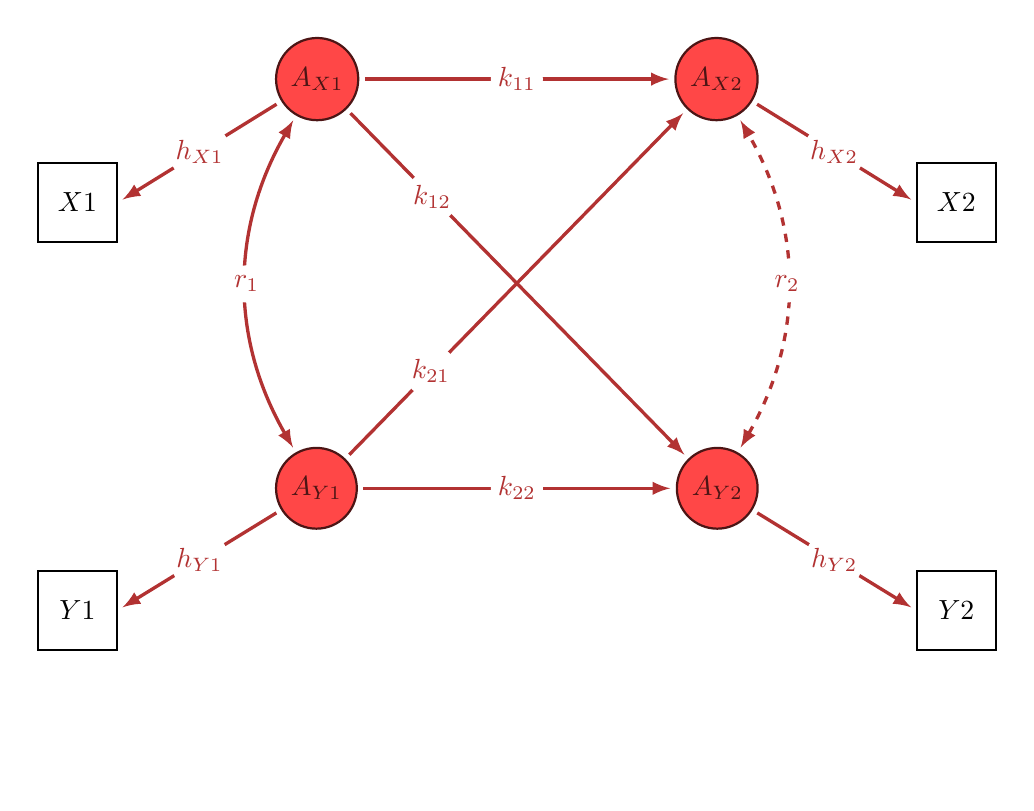
\begin{tikzpicture}[>=latex,node distance = 1.45 cm, minimum size = 1cm]
			\matrix[column sep = 4cm,row sep = 1cm]{
				\node (X11) at (0,0) [manifest] {$X1$};
				\node (C11) [right = 2cm of X11, C] {$C_{X1}$}; 
				\node (A11) [above = 0.5cm of C11, A] {$A_{X1}$};
				\node (E11) [below = 0.5cm of C11, E] {$E_{X1}$}; &
				\node (X12) at (0,0) [manifest] {$X2$};
				\node (C12) [left = 2cm of X12, C] {$C_{X2}$}; 
				\node (A12) [above = 0.5cm of C12, A] {$A_{X2}$};
				\node (E12) [below = 0.5cm of C12, E] {$E_{X2}$}; \\
				\node (X21) at (0,0) [manifest] {$Y1$}; 
				\node (C21) [right = 2cm of X21, C] {$C_{Y1}$}; 
				\node (A21) [above = 0.5cm of C21, A] {$A_{Y1}$};
				\node (E21) [below = 0.5cm of C21, E] {$E_{Y1}$}; &
				\node (X22) at (0,0) [manifest] {$Y2$};
				\node (C22) [left = 2cm of X22, C] {$C_{Y2}$}; 
				\node (A22) [above = 0.5cm of C22, A] {$A_{Y2}$};
				\node (E22) [below = 0.5cm of C22, E] {$E_{Y2}$}; \\
			};
			\begin{scope}[opacity=0, transparency group]
				\path[->,shorten >= 2pt, shorten <= 2pt,line width=1.2,Ccol!70!black]
					(C11) edge (C12)
					(C11) edge (C22)
					(C21) edge (C12)
					(C21) edge (C22)
					(C11) edge (X11.east)
					(C12) edge (X12.west)
					(C21) edge (X21.east)
					(C22) edge (X22.west);
				\path[<->,shorten >= 2pt, shorten <= 2pt, bend left = 30, out = -30, in = -150, line width=1.2,Ccol!70!black]
					(C11) edge (C21)
					(C22) edge [dashed] (C12);
			\end{scope}
			\begin{scope}[opacity=0, transparency group]
				\path[->,shorten >= 2pt, shorten <= 2pt,line width=1.2,Ecol!70!black]
					(E11) edge (E12)
					(E11) edge (E22)
					(E21) edge (E12)
					(E21) edge (E22)
					(E11) edge (X11.east)
					(E12) edge (X12.west)
					(E21) edge (X21.east)
					(E22) edge (X22.west);
				\path[<->,shorten >= 2pt, shorten <= 2pt, bend left = 30, out = -30, in = -150, line width=1.2,Ecol!70!black]
					(E11) edge (E21)
					(E22) edge [dashed] (E12);
			\end{scope}
			\path[->,shorten >= 2pt, shorten <= 2pt,line width=1.2,Acol!70!black]
				(A11) edge node [label] {$k_{11}$} (A12)
				(A11) edge node [label, pos=0.25] {$k_{12}$} (A22)
				(A21) edge node [label, pos=0.25] {$k_{21}$} (A12)
				(A21) edge node [label] {$k_{22}$} (A22)
				(A11) edge node [label] {$h_{X1}$} (X11.east)
				(A12) edge node [label] {$h_{X2}$} (X12.west)
				(A21) edge node [label] {$h_{Y1}$} (X21.east)
				(A22) edge node [label] {$h_{Y2}$} (X22.west);
			\path[<->,shorten >= 2pt, shorten <= 2pt, bend left = 30, out = -30, in = -150, line width=1.2,Acol!70!black]
				(A11) edge node [label] {$r_1$} (A21)
				(A22) edge [dashed] node [label] {$r_2$} (A12);
	\end{tikzpicture}
\end{document}